%
% Example for a student report latex file. Adapt as necessary
%

% the following lines should stay as is
\documentclass[10pt,a4paper,twoside,journal]{IEEEtran}
\usepackage[nocompress]{cite}
\usepackage[pdftex]{graphicx}
\graphicspath{ {images/} }
% some packages that most people use or improve the result
\usepackage[utf8]{inputenc}
\usepackage[english]{babel}
\usepackage{amsmath}
\interdisplaylinepenalty=2500
\usepackage{amssymb}
\usepackage{amsfonts}
\usepackage{amsbsy}
\usepackage{flushend}
\usepackage{siunitx}
\usepackage{array}
\usepackage{xspace}
\usepackage{algorithm}
\usepackage{url}
\usepackage[pagebackref=true,breaklinks=true,colorlinks,bookmarks=false]{hyperref}

% add your additional packages here
\usepackage{lipsum}
%
% DOCUMENT starts here
%
\begin{document}

% configure submission details

% here you can specify the day of submission
\newcommand{\submissiondate}{\today}

% please specify the type of your submission. E.g. Advanced Seminar or Practical
% Laboratory
\newcommand{\submissiontype}{Advanced Seminar}

% give information about when your course happened in form of SEMESTER YEAR,
% e.g. Winter Semester 2016. In addition, specify the "short version", e.g. WS
% 2016
\newcommand{\submissionterm}{Winter Semester 2016}
\newcommand{\submissiontermshort}{WS 2016}

% the full submission title
\newcommand{\submissiontitle}{Student Report Example}
% in case that you have a very long report title, make sure to provide a shorter
% version that can be used in the \markboth command further below. In case your
% topic is short, simply comment the next and uncommented the second line
\newcommand{\submissiontitleshort}{Report Example}
%\newcommand{\submissiontitleshort}{\submissiontitle}

% author list. Make sure that you include your matriculation number in the
% section starting with \thanks. In addition, specify your supervisor(s).
\author{John~Doe, Jane~Roe, and Max~Mustermann%
	\thanks{\textbf{Authors}:
		John Doe (12345678, john.doe@tum.de),
		Jane Roe (87654321, jane.roe@tum.de),
		and Max Mustermann (56794321, max@mustermann.tld)
		% the following includes additional information
		\textbf{Course}: \submissiontype{} \submissionterm{}
		\textbf{Submitted}: \submissiondate{}
		\textbf{Supervisor}: Name Familyname.
		Neuroscientific System Theory (Prof. Dr. J\"org Conradt), Technische
		Universit\"at M\"unchen, Arcisstraße 21, 80333 M\"unchen, Germany.
}}

% both items should look alike and contain a short version of the type of work
% and semester (e.g. Advanced Seminar WS 2016, Project Laboratory SS 2017) and
% your report title. If your title is too long, find a shorter one.
\markboth{\submissiontype{} \submissiontermshort{}: \submissiontitleshort{}}
{\submissiontype{} \submissiontermshort{}: \submissiontitleshort{}}

% this generates the paper title
\title{\submissiontitle}
\maketitle

% write a short abstract to introduce the reader to your work
\begin{abstract}
	Write a short abstract about the topic here. The abstract usually includes a
	very brief introduction to the topic and why it is interesting. This is
	followed by a short description of your work and the conclusions that you
	draw. The abstract is like a teaser to your work. If it is boring, readers
	will stop reading your paper right away. Therefore the abstract should not
	be too long but still include most of the interesting results that you
	discovered.
	The abstract needs to be self-contained. Hence you should not include
	statements that require long explanation. In addition, use only few
	technical terms. Bare in mind that your readers my not be specialists of
	the subject area.
\end{abstract}

%
% Main body follows here. Only capitalize the first word in any title
%
\section{Motivation and Task}
\section{Background and Related Work}

\section{Implementation}


\section{DVS Implementation}
DVS (Dynamic Vision Sensor) is a newly developed instruments for vision data acquisition which imitates the function of human eyes. In this section, we first introduce the DVS theory which we will apply and then modify the data-set into "fake" DVS data-set, which means that we generate  data-set to imitate the DVS-like data-set. Finally we will use these data set to train our fcn network, which is already discussed in \emph{Section \Romannum{3}} .

\subsection{DVS theory}

\begin{figure}
	\centering\textbf{}
	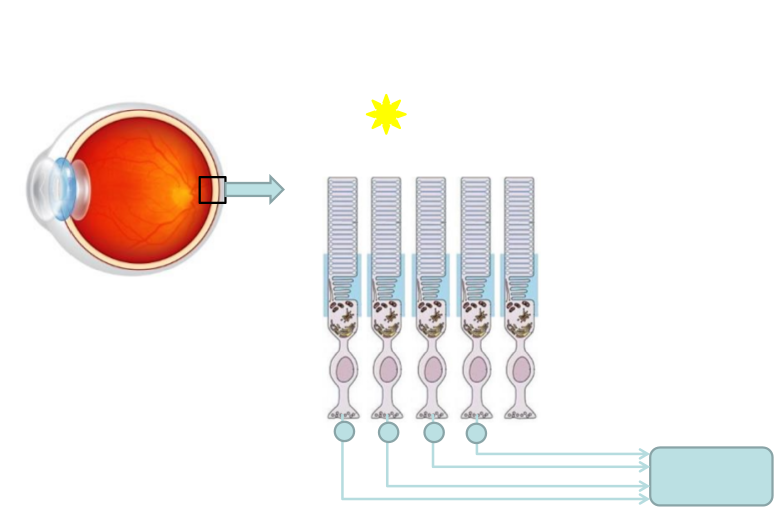
\includegraphics[width=0.4\textwidth]{human_vision.png}
	\caption{Human Vision System\cite{davide}}
	\label{fig:humanvision}
\end{figure}

Nowadays, we are used to record a scene by taking a picture or video. Frame-base devices are dominant in daily life. It is natural that we record a piece of event by filming them frame by frame no matter what devices we use, like CCD or CMOS. The advantages are obvious, they have small simole pixels, leading to high resolution, large fill factor and low imager cost. The output format is understandable and this is the basis for many years of research in computer vision. However, frame-base architecture has high cost when storing information where the intensity of pixels never change based on a series of snapshots taken at a constant rate. The latency of the vision requires high-speed frame rate, which results massive output-data. \cite{lichtsteiner2008128}. The basic problem of frame-based architecure is the hight latency and temporal discretization. The average latency of robot vision algorithm is about 50-200ms, which constrains the development of robotics in high-speed scenarios, such as autonomous driving or unmanned aerial vehicle.

Inspired by human vision system, seen in Figure \ref{fig:humanvision}, the retinal outputs are massively parallel and data driven. The neurons of the retina do not spike all at the same time. In vertebrates, the decisions on when to quantize are made by the ganglion cells that project to the brain and that send their information in the form of digital events which occur in continuous time.\cite{liu2015event} 

Therefore, dynamic vision sensor (DVS) is designed to meet the challenge of the processing speed with traditional on-board cameras. DVS outputs asynchronous evens at microsecond resolution, while traditional camera outputs frames frames at fixed time intervals. An event is generated each time a single pixel changes value. If the change in brightness is larger than \emph{C} then, an \emph{on event} will be generated, if smaller than \emph{-C}, \emph{off event} will be produced, seen in Figure \ref{fig:dvsscheme}. However, these DVS generated "pictures" are quite different from common-used pictures, which is based on the frame. To integrate DVS into training FCN, there is still a lot of work to to in data reprocessing. By accumulate all events occurred in a time interval $\Delta t$, we can visualize the event stream. Such as we accumulate all events of a rotating dot in a time interval, then in visualization, it could be a circle. When the time increases, the brightness of this circle will be darker. Based on that simple rule, we can thus in next section to produce a "fake" DVS data-base using common dataset used to train ConvNets.
\begin{figure}
	\centering\textbf{}
	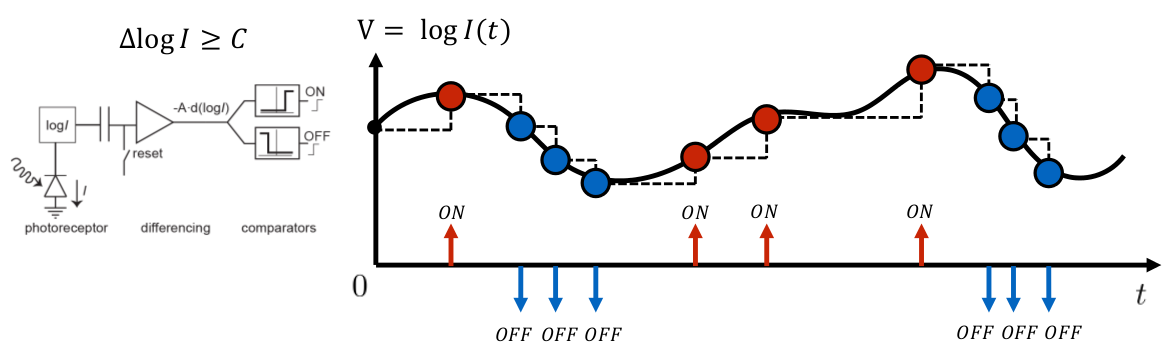
\includegraphics[width=0.5\textwidth]{dvsschem.png}
	\caption{DVS Operation Principle\cite{davide}}
	\label{fig:dvsscheme}
\end{figure}

\subsection{DVS Dataset}

\begin{figure}
\centering
\subfigure[DVS Image with clutter]{
\begin{minipage}[b]{0.2\textwidth}
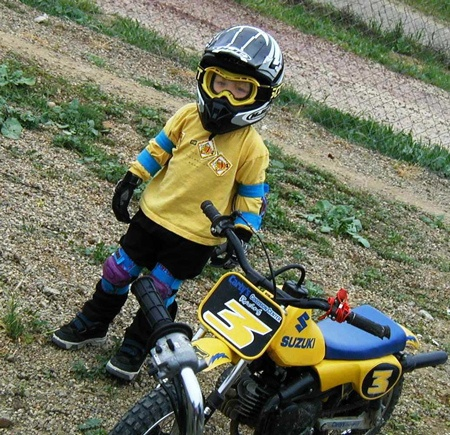
\includegraphics[width=0.9\textwidth]{1.jpg} \\
\label{fig:withclutter}
\\
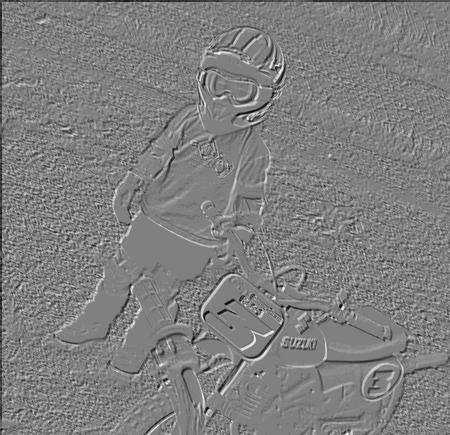
\includegraphics[width=0.9\textwidth]{1_DVS.jpg}
\end{minipage}
}
\subfigure[DVS Image without clutter]{
\begin{minipage}[b]{0.2\textwidth}
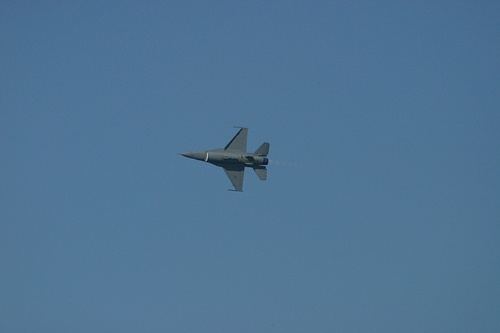
\includegraphics[width=1.2\textwidth]{2.jpg} 
\label{fig:withoutclutter}\\
\\
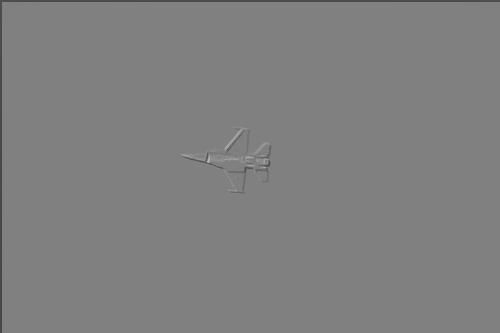
\includegraphics[width=1.2\textwidth]{2_DVS.jpg}
\end{minipage}
}
\caption{DVS Data Set}
\label{fig:dvsdata}
\end{figure}

Here we transfer data set consisted of over 10000 pictures from +++++ into fake event base data set, seen in Figure \ref{fig:dvsdata}. We first scale the images into gray images A. Then shift each image to a random direction to produce an "event" in image B. It imitates the motion of an object in the picture. Next, we subtract the gray scaled image A with shifted image B, which results a change over pixels. We produce "events" by means of assuming a threshold $C$. If the change of pixel intensity is larger than $C$, then it is an \emph{on event}. On the  contrary, if the change of pixel intensity is the smaller than $-C$, then is is an \emph{off event}. Within the interval $[-C,C]$, there exits no event. The Equations are derived as follows
\begin{equation}
    I_{i,j}^{new} =
    \begin{cases}
    \frac{\Delta I_{i,j}}{2(1-C)}+\frac{1}{2(1-C)} &\mbox{$\Delta I_{i,j}\in [-1,-C]$ \emph{off event}}\\
    \frac{1}{2} &\mbox{$\Delta I_{i,j}\in [-C,C]$ \,\emph{no event}}\\
    \frac{\Delta I_{i,j}}{2(1-C)}+\frac{1-2C}{2(1-C)} &\mbox{$\Delta I_{i,j}\in [C,1]$\,\,\,\,\,\emph{on event}}
   \end{cases}
  \end{equation}
where $I_{i,j}^{new}$ is the resulting intensity of the corresponding pixel $(i,j)$, $\Delta I_{i,j}$ is the difference of intensity of the same pixel $(i,j)$ from image A and image B. Note that, in programme, we scale the intensity interval into $[0,1]$.

However, this procedure will make every single thing in the picture moving in a certain direction. If the scene we take has no so much clutter, the result images is quite smoothing, on contrast, if the scene has so much clutter like Image \ref{fig:withclutter}, then the resulting image will be filled by "events". Thus, DVS data can not deal with the scene with much clutter, because it can not give us "useful " information about the object. However, like the Figure \ref{fig:withoutclutter}, the outline of the object "airplane" is obvious. If we use real DVS data, it can be clearly inferred that the direction of the flight without any other redundancy

\subsection{Training based on DVS data set}
After generating the data-set we use in FCN network previously, we can now train the network based on the DVS data set. During training, we find that the loss function can not converge. Seen in Figure.

% \begin{figure*}
%     \centering
%     \subfigure{
%     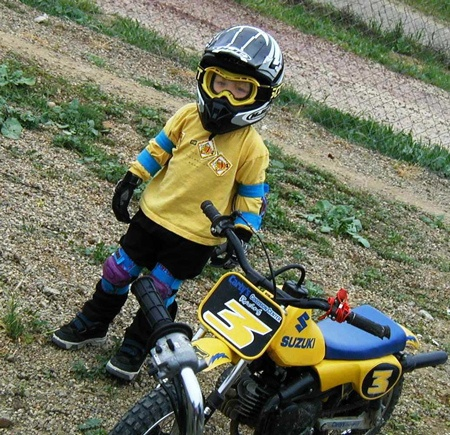
\includegraphics[width=0.25\textwidth]{1.jpg}
%     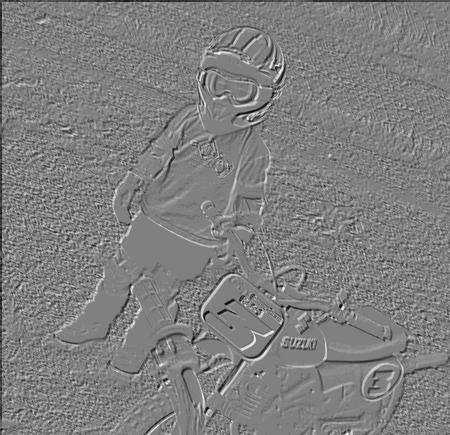
\includegraphics[width=0.25\textwidth]{1_DVS.jpg}
%     \caption{DVS with clusters}
%     }
    
%     \subfigure{
    
%     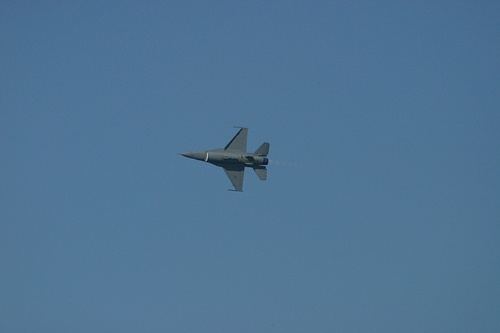
\includegraphics[width=0.3\textwidth]{2.jpg}
%     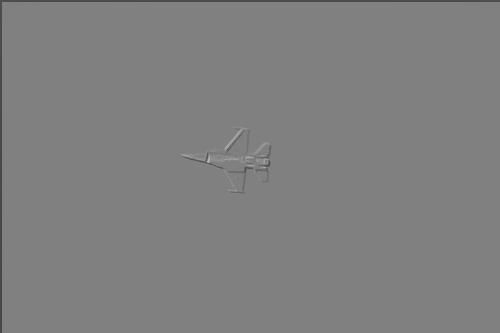
\includegraphics[width=0.3\textwidth]{2_DVS.jpg}
%     \caption{DVS without clusters}
%     }
% \end{figure*}

%\begin{figure}
%	\centering
%	\includegraphics[width=0.4\textwidth]{}
%\end{figure}


\section{Working with this report template}

\IEEEPARstart{W}{riting} a report is almost straightforward as long as you are
properly prepared. Make sure that you found a suitable structure for your
report. For instance, you could split up a report into the following sections:

\begin{enumerate}
	\item Introduction
	\item Related work
	\item Implementation details
	\item Experiments and evaluation
	\item Conclusion.
\end{enumerate}

However you may have to adapt to the report you are writing. An advanced seminar
usually does not contain experiments and evaluation, but you wish to show
details about one references paper that you found.

If you're unsure how to structure your report, contact your supervisor. Together
with your supervisor you should be able to figure out how to best organize your
manuscript.

Then the remaining task mostly consists of writing. Writing a good paper only
comes with experience, though, and an understanding how a good paper should be
structures. An excellent overview about the latter issue can be found in
\cite{katzoff1964}.

\section{Additional \LaTeX{} packages}

You are free to use any additional packages that you require. There are some
caveats, though. Make sure to include packages that do not ship with standard
\LaTeX{} distributions in your final submission. Most of the important packages
are included already in the preamble of this document, though.


\section{Spelling}

Before handing in your thesis, even for an intermediate review, please perform a
spellcheck and correct grammar mistakes. The report is not meant to be a
narrative text. Please stick to neutral and technical style and avoid subjective
or biased expressions or adjectives/adverbs such as \emph{obviously, always,
very, especially well, actually, so-called etc}. Scientific writing is about
precision and you should underpin your statements factually, not soften them
with unnecessary qualifiers.

%Sometimes you have a wide figure or environment. Inclusion can be achieved using
%the \texttt{figure*} environment as used in Figure \ref{fig:twocolumnfigure}.
%\begin{figure*}
%	\centering
%	\fbox{\rule{0pt}{2cm} \rule{1.0\linewidth}{0pt}}
%	\caption{A wide figure.}
%	\label{fig:twocolumnfigure}
%\end{figure*}

\section{Technical details}

In the following we will give you some short information about how you should
typeset mathematical equations and set tables or figures. If you require more
information about the topics then first try to find answers on the Internet, and
only if you did not figure out how to solve your issue, contact your supervisor.

\subsection{Mathematical equations an}

In case you have to typeset equations make sure that all equations are numbered.
The following example shows how to do so

\begin{equation}
	E = mc^2
\end{equation}

Sometimes you wish to align equations. This is possible with the (already
included) \texttt{align} package. The example in Equation \ref{eq:lotkavolterra}
which gives the Lotka--Volterra, or predator-prey equations, shows how to use
it.

\begin{align}\label{eq:lotkavolterra}
	\frac{dx}{dt} &= \alpha x - \beta x y \\
	\frac{dy}{dt} &= \delta x y - \gamma y
\end{align}

\subsection{Figures, tables, algorithms}

Most reports need to include one of the mentioned objects. There are suitable
environments for each of them. If you are interested in typesetting algorithms,
have a look at the packages \texttt{algorithmic} and \texttt{algorithmx}. Make
sure that all algorithms are well formatted and clearly understandable!

Figures are included using the \texttt{figure} environment. All graphics should
be centered.  Please ensure that any point you wish to make is resolvable in a
printed copy of the paper. Resize fonts in figures to match the font in the
body text, and choose line widths which render effectively in print. An example
%is shown in Figure \ref{fig:onecolumnfigure}.
%\texttt{includegraphics} will include the respective file.
%\begin{figure}
%	\centering
%	\fbox{\rule{0pt}{2cm} \rule{1.0\linewidth}{0pt}}
%	\caption{Always add a short caption to your figures.}
%	\label{fig:onecolumnfigure}
%\end{figure}


\section{Submission}

When submitting your final report, make sure to include all files that are
required to build the PDF from source. This includes all bibliography files and
\LaTeX{} files. In addition, don't forget to include all figures. If you
performed an evaluation on a dataset you should include this data as well. For
project laboratories or seminars that produced source code, this should be
shipped with your final submission as well. If you prefer to keep your code
secret, contact your supervisor.

%
% If you wish to put your work under a specific license, your free to do so. You
% are not obliged, so you can remove the following section if you wish to.
%
\section*{License}
\markright{LICENSE}
This work is licensed under the Creative Commons Attribution 3.0 Germany
License. To view a copy of this license,
visit \href{http://creativecommons.org/licenses/by/3.0/de/}{http://creativecommons.org} or send a letter
to Creative Commons, 171 Second Street, Suite 300, San
Francisco, California 94105, USA.


% each report should include all references that you cite in the work. Make sure
% that you include all references!
\bibliographystyle{ieee}
\bibliography{bibliography}

\end{document}
